\paragraph*{Unfolding of the matrix power.}
%The general idea behind the  unfolding operation 
%\begin{align*}
%\ranked{
%    \unfoldsmall : \shallowterm {(\reduce k   \Sigma)} {\Gamma^k} \to \reduce 1 (\shallowterm \Sigma \Gamma)
%}
%\end{align*} 
%is to eliminate a $k$-fold by matching it with a $k$-th power. 
%The unfolding operation is explained in the following picture for $k=2$: 
%        \begin{center}
%        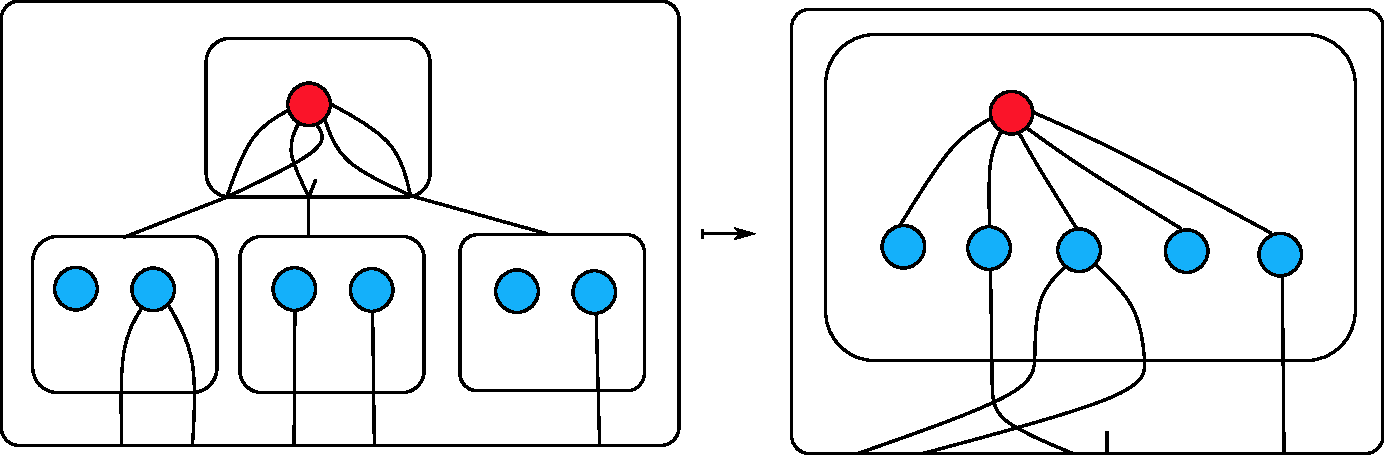
\includegraphics[scale=.36]{shallow-unfold.pdf}
%        \end{center}

\begin{figure}[]
    \mypic{101}    
    \caption{Unfolding the matrix power}
    \label{fig:unfold}
\end{figure}
We now explain the unfolding operation 
\begin{align*}
    \ranked{\unfold : \tmonad \reduce k \overbrace{(\rSigma \otimes \cdots \otimes \rSigma)}^{\black{\text{$k$ times}}} \to  \reduce k \overbrace{(\tmonad\rSigma \otimes \cdots \otimes \tmonad\rSigma)}^{\black{\text{$k$ times}}}\ }.
    \end{align*}
We begin by introducing some notation.
%Roughly speaking, the several trees are the contents of registers in a register automaton.
%, and the single tree that represents them is the computation tree of the register automaton.  We then show that several trees stored in a computation  can be unfolded in a derivable way. 
\miktodo{mention the restriciton on monotone twists}

\begin{definition}
    [Matrix power] For $k \in \set{1,2,\ldots}$ define the $k$-th matrix power\footnote{
        The name  matrix power is based the matrix power in  universal algebra (for the latter, see~\cite{Taylor1975} or~\cite{szendrei1990simple}). Roughly speaking, the restrictions that we place on the original definition correspond to the single-use and monotone conditions from Definition~\ref{def:stt}. 
     } of a ranked set $\rSigma$ 
to be 
\begin{align*}
 \mati k \rSigma \quad \eqdef \quad \ranked{\reduce k \rSigma^k}.
\end{align*}
\end{definition}
In terms of the matrix power notation, the type of the unfolding function is $\ranked{\tmonad \mati k{\Sigma} \to \mati k{( \tmonad \Sigma)}}$. 
Here is a picture of a  binary element in the third matrix power:
\mypic{102}
An $n$-ary  element of the $k$-th matrix power  can be seen as having a group of $k$ incoming edges, and each of the $n$ ports can be seen as a group of $k$ outgoing edges. The idea  unfolding  is that it matches the $k$ incoming edges in a node with the $k$ outgoing edges in the parent port; it also removes the unreachable nodes. This is illustrated in Figure~\ref{fig:unfold}. The unfolding operation will be discussed in more detail in Section~\ref{sec:stt-derivable}, and a formal definition is given in the appendix.


% Suppose that the input is 
% \begin{align*}
% (\tensorpair{a_1,\ldots,a_k}/f)\tensorpair{t_1,\ldots,t_n} \in 
% \end{align*}
% First apply the unfold operation to the smaller trees $t_1,\ldots,t_n$, yielding trees
% \begin{align*}
% \tensorpair{t_{11},\ldots,t_{1k}}/f_1 \quad \cdots \quad  \tensorpair{t_{n1},\ldots,t_{nk}}/f_n
% \end{align*}
% For $i \in \set{1,\ldots,k}$ construct a term $s_i$ as follows. The root label is $a_i$. If the arity of $a_i$ is $n_i$, then let $t_{ij}$ be the tree 
% For two ranked sets $\rSigma$ and $\rGamma$, define 
% \begin{align*}
% \shallowterm \rSigma \rGamma \quad \eqdef   \quad \ranked{\coprod_{\black{a \in} \rSigma} } \overbrace{\ranked{\Gamma \otimes \cdots \otimes \Gamma}}^{\text{arity of $a$ times}}
% \end{align*}
% \begin{align*}
%     \ranked{
%         \xymatrix{
%             \shallowterm{\mati k \rSigma} {\mati k \rGamma}  \ar[r] & \mati k {(\shallowterm \Sigma \Gamma)}.
%         }
%     }
% \end{align*}
% \begin{align*}
% \tmonad \rSigma = \redset{ \portletter} + \shallowterm \rSigma {\tmonad \rSigma}
% \end{align*}


% to be the set of terms over alphabet $\rSigma + \rGamma$, where the 
% % , this operation of determining the dependency tree is what we call \emph{unfolding}. We illustrate it by the following example 
% % \begin{center}
% % 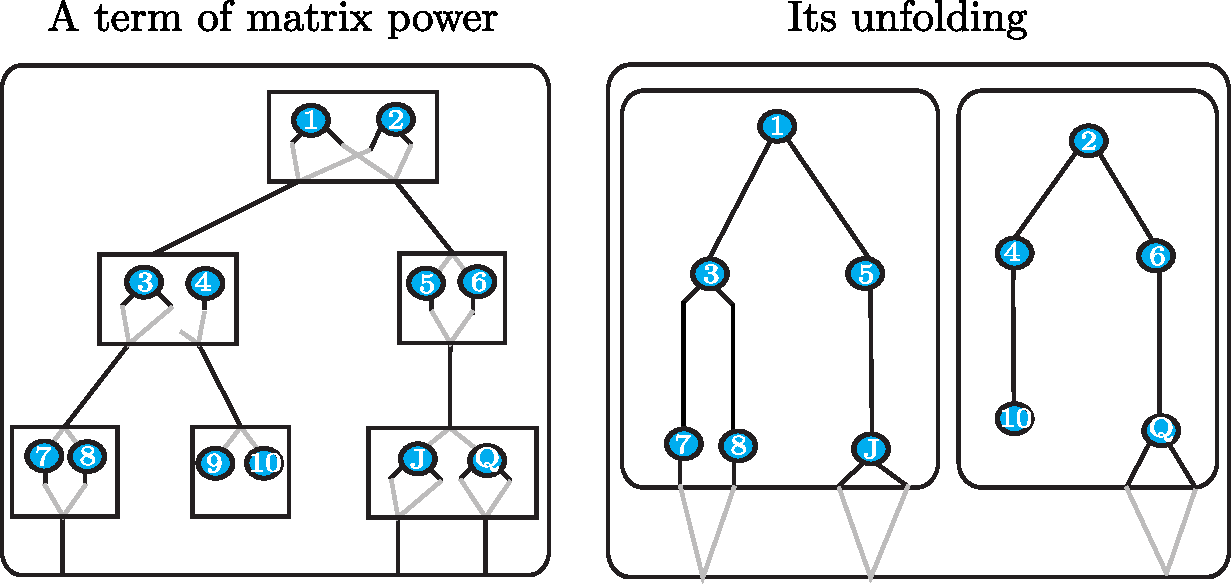
\includegraphics[scale=.38]{unfold-matrix-power}
% % \end{center}
% %  which is defined as follows by induction on the size of the input term. 
% If the input is an empty term, then the output is this term:
% \begin{center}
% \includegraphics[scale=.3, page=83]{pics.pdf}
% \end{center}
% % Otherwise, if the input is a nonempty term $(a_1,\ldots,a_k)/f)(t_1,\ldots,t_n)$. 
% Apply unfolding inductively, yielding 
% For $i \in \set{1,\ldots,k}$ define $s_i$ to be the tree where the root label is $a_i$, and the children are obtained ... 

% Consider an edge in the tree $t$, which connects either a node with one of its children, or a node with one of the ports. For $i \in \set{1,\ldots,k}$, define the $i$-th source of the edge to be the node ; likewise define the $i$-th target of the edge to be the $i$-th subnode of $s$.  For a node $x$ in $t$ and $i \in \set{1,\ldots,k}$, define the $i$-th subnode of $x$ to be the label (from $\rSigma$) in the $i$-th coordinate of the label of $x$.  For a subnode, define its \emph{outgoing edge} to be the edge of the tree 

% Define a \emph{inport} of $s$ to be a pair (node of $s$, number in $\set{1,\ldots,k$}). Define an \emph{outport} to be a pair (node $s$, number in $\set{1,\ldots,k}$, number in $\set{1,\ldots,\text{arity of $s$}$}). 

% \begin{align*}
% \underbrace{\text{(nodes in $s$)} \times \set{1,\ldots,k}}_{\text{sub-nodes}} 
% \qquad
% \underbrace{\text{(edges in $s$)} \times \set{1,\ldots,k}}_{\text{sub-edges}}
% \end{align*}
% For a sub-node $(v,i)$, define its label to be the label in $\rSigma$ of the $i$-th coordinate in the label of $v$. Define the arity of the sub-node to be the arity of its label. If a sub-node has arity $n$, and $j \in \set{1,\ldots,n}$, then the $j$-th out-going sub-edge of the sub-node is defined in the natural way. 


% Consider an  element
% \begin{align*}
% (a_1,\ldots,a_k)/f  
% \end{align*}

% \begin{align*}
% \coprod_{i \in \set{1,\ldots,k}} \set{1,\ldots,\text{arity of $a_i$}} \qquad \to \qquad \set{1,\ldots,n} \times \set{1,\ldots,k}
% \end{align*}
% For $i \in \set{1,\ldots,k}$ and a node node $v$ in the tree $s$ which has label $(a_1,\ldots,a_k)/f$. For $j \in \set{1,\ldots,\text{arity of $a_i$}}$. Let define the $j$-th child of to be the 

% Define a \emph{sub-edge} to be a pair (edge in $s$, number in $\set{1,\ldots,k}$). Define a \emph{sub-node} to be a pair (node in $s$, number in )

% then the output is obtained by first applying unfolding to to the smaller terms $t_1,\ldots,t_n$, and then applying the following derivable function, which we call \emph{shallow unfold}. 
% \begin{align*}
%     \ranked{
%         \xymatrix{
%             \shallowterm{\mati k \rSigma} {\mati k \rGamma}  \ar[r] & \mati k {(\shallowterm \Sigma \Gamma)}.
%         }
%     }
% \end{align*}
% Here is a picture of unfolding for shallow terms:
% \begin{center}
% 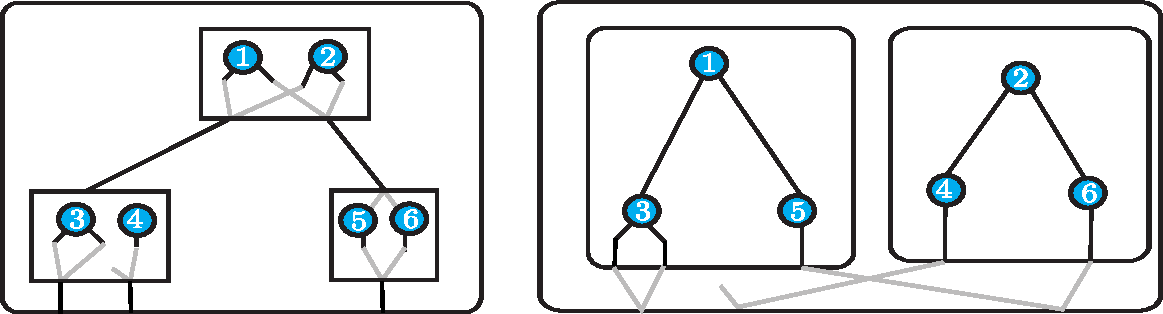
\includegraphics[scale=.4]{unfold-shallow}
% \end{center}